\Chapter{Resultaten\label{hfdst-resultaten}}

In dit hoofdstuk zal het ASIC ontwerp van de schakeling die in \refhfdst{hfdst-implementatie} beschreven werd van naderbij bestudeerd worden. Daarbij zal gekeken worden naar de oppervlakte van de schakeling, het verbruik en de maximum bereikbare kloksnelheid $f_{\text{max}}$. Er zal onderzocht worden wat het effect van de verschillende voorgestelde optimalisaties is op al deze parameters. Ten slotte zal het ontwerp vergeleken worden met reeds bestaande implementaties.

Het ontwerp werd geprogrammeerd in GEZEL \cite{gezel}. Simulaties en compilatie naar VHDL werden uitgevoerd met GEZEL 2.0. De optimalisaties werden doorgevoerd in de VHDL code, aangezien GEZEL dit niet toelaat. Alle ontwerpen werden gesynthetiseerd met behulp van Synopsys Design Vision. De gebruikte bibliotheek was de \emph{$0.13 \mu m$ low leakage} bibliotheek van Faraday Technology \cite{cell-databook}. Het werd de software verboden flip-flops met test ingangen te gebruiken. De maximale oppervlakte werd ingesteld op nul, wat als netto effect een resultaat met minimum oppervlakte gaf. Verder werd voor het kloksignaal een frequentie van 100kHz gedefini\"eerd.

De grootte van alle resultaten wordt uitgedrukt in gates. Dit laat toe te vergelijken met andere resultaten die in de literatuur terug te vinden zijn.

Voor de resultaten in verband met energieverbruik worden steeds twee waarden gegeven. De eerste waarde, dynamisch verbruik, geeft weer hoeveel vermogen verbruikt wordt door veranderende CMOS in- en uitgangen. De tweede waarde, leakage verbruik, is verbruik dat voorkomt zelfs indien een transistor niet geleidt. De impact hiervan hangt onder meer af van de gebruikte bibliotheek.

De beide waarden moeten met een stevige korrel zout genomen worden. Het is voor het synthese programma zeer moeilijk hier een nauwkeurige schatting voor te geven. Zolang twee schakelingen echter met dezelfde software, bibliotheek en parameters werden gesynthetiseerd, zijn relatieve vergelijkingen mogelijk. Stel bijvoorbeeld dat het verbruik van ontwerp A geschat wordt op $200 nW$ en dit van ontwerp B op $100 nW$. Indien er dan voldaan is aan de voorgenoemde voorwaarden, zal het effectief verbruik van B ongeveer de helft zijn van A. Het is dus in het algemeen niet aangeraden vergelijkingen omtrent verbruik te maken met andere bestaande ontwerpen aan de hand van de waarden gegeven in dit hoofdstuk.

% TODO: Blijft leakage constant bij hogere kloksnelheid?

Indien gewenst kan het verbruik voor hogere kloksnelheiden geschat worden. Gegeven de formule voor het dynamisch verbruik van een CMOS schakeling:
\[P_d = V^2 \cdot C \cdot f\]
en het leakage verbruik $P_l$, kan men dus het totale verbruik omrekenen naar dat van een willekeurige kloksnelheid via
\[P' = \frac{P_d \cdot f'}{100 000} + P_l.\]

\section{Basisimplementatie \& register optimalisaties\label{section-resultaten-basisimplementatie}}

Het synthetiseren van de meest eenvoudige implementatie, zonder enige optimalisaties aan de registers en met slechts \'e\'en MALU in de $\mathbb{F}_{2^m}$ kern, geeft de resultaten in \reftbl{tabel-resultaten-basis}.

\begin{table}[h]
	\caption{Syntheseresultaten voor de basis implementatie}
	\label{tabel-resultaten-basis}

	\centering
	\begin{tabular}{|l|l|l|l|}
		\hline
		\multirow{2}{*}{Opp. (gates)}	& \multicolumn{2}{c|}{Verbruik @ 100kHz ($nW$)}	& \multirow{2}{*}{$f_{\text{max}}$ (MHz)}\\
		\cline{2-3}
		& Dynamisch	& Leakage	& \\
		\hline
		$31\:943$	& 515	& 134	& 53.22\\
		\hline		
	\end{tabular}
\end{table}

Deze resultaten zullen nu vergeleken worden met de verschillende register optimalisaties. Bij de implementaties van clock gating wordt steeds ook de reset ingangen van zoveel mogelijk registers verwijderd. De synthese resultaten voor de vier verschillende optimalisaties worden gegeven in \reftbl{tabel-resultaten-optimalisaties}. Zoals verwacht verbruiken al deze resultaten minder dan de niet-geoptimaliseerde versie. De versies met clock gating (CG $n$) implementeren de schakelingen in de volgorde waarin ze voorkomen in \refsect{subsectie-implementatie-optimalisatie-clock-gating}. Voor elke parameter wordt aangegeven hoeveel deze beter is dan in de niet-geoptimaliseerde versie. Ter verduidelijking zijn de oppervlakte en het totale verbruik van deze resultaten ook nog eens uitgezet in \reffig{figuur-resultaten-m1}.

\begin{table}[h]
	\caption{Syntheseresultaten voor de register optimalisaties}
	\label{tabel-resultaten-optimalisaties}

	\centering
	\begin{tabular}{|l|lr|lr|lr|lr|}
		\hline
		& \multicolumn{2}{l|}{\multirow{2}{*}{Opp. (gates)}}	& \multicolumn{4}{c|}{Verbruik @ 100kHz ($nW$)}	& \multicolumn{2}{l|}{\multirow{2}{*}{$f_{\text{max}}$ (MHz)}}\\
		\cline{4-7}
		&	& & \multicolumn{2}{l|}{Dynamisch}	& \multicolumn{2}{l|}{Leakage}	& &\\
		\hline \hline
		Basis			& $31\:943$	& & 515	& 	& 134 & 	& 53.22 & \\
		\hline
		Geen reset	& $33\:221$	& 1\%	& 473	& 5\%	& 134 & 0\%	& 54.08	& 2\%\\
		CG 1			& $30\:481$	& 1\%	& 104	& 5\%	& 117	& 5\%	& 47.73	& 5\%\\
		CG 2			& $30\:481$	& 1\%	& 104	& 5\%	& 117	& 5\%	& 47.73	& 5\%\\
		CG 3			& $30\:481$	& 1\%	& 104	& 5\%	& 117	& 5\%	& 47.73	& 5\%\\
		\hline		
	\end{tabular}
\end{table}

\begin{figure}[h]
	\centering
		\fbox{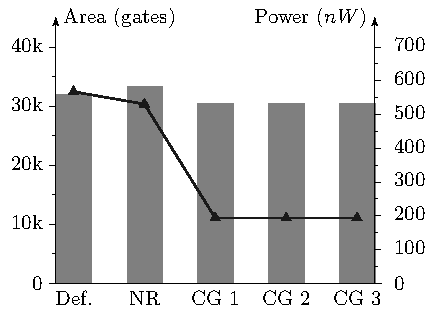
\includegraphics[width=8cm]{results-m1}}
		\caption{Syntheseresultaten voor de basis implementatie met en zonder register optimalisaties\label{figuur-resultaten-m1}}
\end{figure}

\section{Meerdere MALU's\label{sectie-resulaten-malus}}

Mits de toevoeging van extra MALU's is het mogelijk de totale rekeningtijd drastisch te verlagen (zie \refsect{subsectie-implementatie-gf2m-versnelling}). Hoewel het gebruik van meerdere MALU's de uiteindelijke schakeling vergroot en dat dus enigszins in gaat tegen de originele doelstelling, wordt hier toch onderzocht in welke mate de interessante parameters hierdoor juist worden be\"invloed. Er kan dan een afweging gemaakt worden tussen het gebruik van een schakeling met \'e\'en MALU op hogere kloksnelheid versus \'e\'en met meerdere MALU's aan een lagere kloksnelheid. De eerste schakeling zal kleiner zijn, maar waarschijnlijk wel meer verbruiken dan de tweede.

De totale berekeningstijd $t = \frac{c}{f}$ kan bepaald worden in functie van het aantal benodigde klokcycli $c$ en het aantal MALU's $d$:
\[c = 27058 + 2993 \cdot \left\lceil \frac{163}{d} \right\rceil,\]
waarbij 2993 het aantal vermenigvuldigingen is dat dient uitgevoerd te worden en de tweede term in de vermenigvuldiging het aantal klokcycli is dat een vermenigvuldiging kost. In \reftbl{tabel-resultaten-multi-cycles} wordt voor enkele waarden getoond hoeveel klokcycli nodig zijn om een berekening te voltooien. In \reffig{figuur-resultaten-multi-cycles} wordt hetzelfde weergegeven, maar dan voor elke $d$ van 1 t.e.m.\ 163. Het is duidelijk dat de tijdsbesparing waar extra MALU's voor zorgen vrij snel teniet wordt gedaan door het aantal cycli dat niet door $d$ be\"invloed wordt.

\begin{table}[h]
	\caption{Aantal klokcycli $c$ nodig voor \'e\'en pairing i.f.v.\ aantal MALU's $d$}
	\label{tabel-resultaten-multi-cycles}

	\centering
	\begin{tabular}{|l|l|l|l|l|l|l|l|l|}
		\hline
		$d$	& 1	& 2	& 3	& 4	& 6	& 8	& 16	& 32\\
		\hline
		$c$	& $514\:917$	& $272\:484$	& $191\:673$	& $149\:771$	& $110\:862$	& $89\:911$	& $59\:981$	& $45\:016$\\
		\hline		
	\end{tabular}
\end{table}

\begin{figure}[h]
	\centering
		\fbox{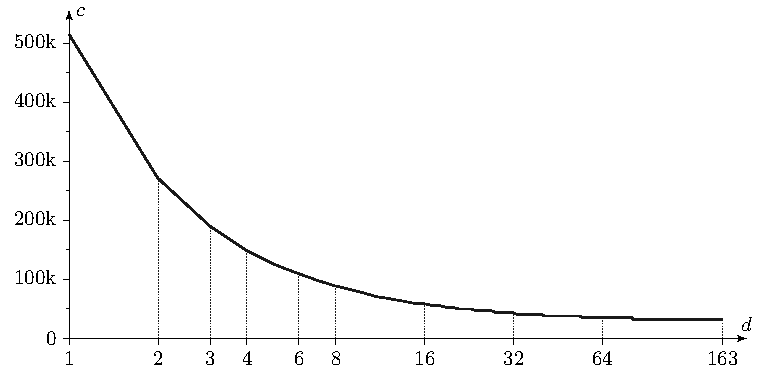
\includegraphics[width=\textwidth]{results-multi-cycles}}
		\caption{Aantal klokcycli $c$ nodig voor \'e\'en pairing i.f.v.\ aantal MALU's $d$\label{figuur-resultaten-multi-cycles}}
\end{figure}
